\documentclass[aspectratio=169]{beamer} %[handout]
\mode<presentation>
\definecolor{links}{HTML}{0101DF}
\hypersetup{colorlinks,linkcolor=,urlcolor=links}
\setbeamercovered{transparent}
\usetheme[hideothersubsections]{Hannover}
\usecolortheme{fly}
\usenavigationsymbolstemplate{}
\usepackage{lmodern}
\renewcommand{\familydefault}{\sfdefault}

%%language
\usepackage[utf8]{inputenc}
\usepackage[T1]{fontenc}
\usepackage{ngerman}
\usepackage[ngerman,iso]{isodate}
%\usepackage{eurosym}
\hyphenation{}

\setbeamertemplate{section in toc}{\hspace*{1em}\inserttocsection}

\usepackage{graphicx}
\usepackage{multicol}
\usepackage{wallpaper}

%\usebackgroundtemplate{\only<2->{
%    \rotatebox{90}{\makebox[5.7cm][l]{}}
%    \makebox[\textwidth][r]{\includegraphics[height=2.6cm]{pic/FFW_Wassel.jpg}}
%}}
\begin{document}
\title{Feinstaub in Lehrte}
\subtitle{Projektausschnitt von \href{http://www.luftdaten.info}{luftdaten.info}}
\author{Dr. H-J. Dankert, S. Frenger}
\institute{luftdaten.info} 
\date{2018-01-23} 

\frame{\titlepage} 

\begin{frame}{Inhalt}
  \begin{multicols}{2}
    \tableofcontents
  \end{multicols}
\end{frame}

\section{Feinstaub}

\subsection{Gesundheitsrisiken}
\begin{frame}{Feinstaub}
  \begin{itemize}
  \item PM10 kann in die Nasenhöhle
  \item PM2.5 kann in Bronchien und Lungenbläschen 
  \item noch kleinere in Lungengewebe und Blutkreislauf
  \item Pollen
  \item Feuer
  \end{itemize}
\end{frame}

\subsection{Gesetz}
\begin{frame}{Gesetz}
  \begin{itemize}
  \item \href{https://www.umweltbundesamt.de/daten/luft/feinstaub-belastung}{umweltbundesamt.de}:
    Seit 2005 darf eine PM10-Konzentration von 50 Mikrogramm pro Kubikmeter (µg/m³) im Tagesmittel nur an höchstens 35 Tagen im Kalenderjahr überschritten werden.
  \end{itemize}
\end{frame}


\subsection{Ursachen}
\begin{frame}{Ursachen}
  \begin{itemize}
  \item Verkehr
    \begin{itemize}
    \item Abgase
    \item Bremsen
    \item Stau, Umleitungsverkehr, Ferienverkehr
    \end{itemize}
  \item Heizung
  \item Pollen
  \item Feuer
  \end{itemize}
\end{frame}

\subsection{Stuttgart}
\begin{frame}{Stuttgart}
  \begin{itemize}
  \item open Data
  \item Stuttgart im Tal
  \item Feinstaub messen: teuer?
  \item Projektstart 2015
  \end{itemize}
\end{frame}

\subsection{Bausatz}
\begin{frame}{\href{http://luftdaten.info/feinstaubsensor-bauen/}{Bausatz}}
  \begin{itemize}
  \item MiniPC mit WLAN: NodeMCU ESP8266
  \item Feinstaubsensor: SDS011
  \item Temperatur & Luftfeuchtigkeit: DHT22 
  \item Wetterschutz: HT Bogen
  \item Verbindung: USB-Ladekabel, WLAN
  \end{itemize}
  \begin{center}
    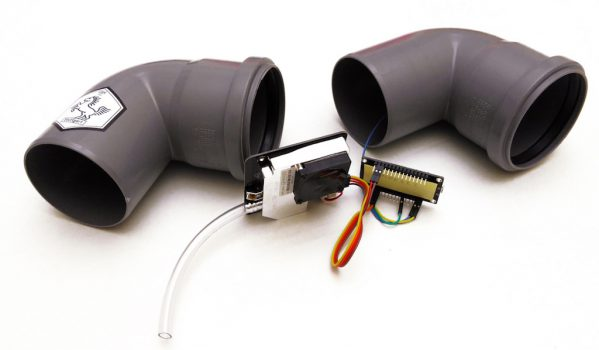
\includegraphics[width=6cm]{../screenshots/Feinstaub-Sensor-Bausatz-e1479558693357.jpg}
  \end{center}
\end{frame}

\subsection{Aktuelle Nachrichten}
\begin{frame}{Aktuelle Nachrichten}
  \begin{itemize}
  \item 17-07-27 Augsburger \href{http://www.augsburger-allgemeine.de/panorama/In-Stuttgart-droht-jetzt-ein-Diesel-Fahrverbot-id42204121.html}{Stuttgart droht Diesel-Fahrverbot}
  \item 17-09-16 Wirtschaftsn \href{https://deutsche-wirtschafts-nachrichten.de/2017/09/16/feinstaub-belastung-vielen-staedten-drohen-fahrverbote/}{Vielen Städten droht Fahrverbot}
  \item 17-09-19 Euronews \href{http://de.euronews.com/2017/09/19/der-deutsche-autowahlkampf}{Deutscher Autowahlkampf}
  \item 17-11-06 Stadt Lehrte referenziert Feinstaub-Projekt \href{http://piratenpartei-lehrte.de/2017/09/11/feinstaub-in-lehrte/}{Feinstaub in Lehrte}
  \item 18-01-04 Silvester \href{https://sbamueller.wordpress.com/2018/01/01/silvester-und-feinstaub/}{Blogger}
  \item 18-01-18 Welt \href{https://www.welt.de/wirtschaft/article172580444/Fahrverbote-kann-Deutschland-kaum-noch-verhindern.html}{Fahrverbote in Deutschland kaum zu verhindern}
  \end{itemize}
\end{frame}

\subsection{Lehrte}
\begin{frame}{Interessant für Lehrte?}
  \begin{itemize}
  \item ISEK: Innen- vor Außenbebauung infragestellen?
  \item Kleingärten
  \item grüne Lunge
  \item soll Baugebiet weichen
  \item verträglich?
  \end{itemize}
\end{frame}

\subsection{Teilnehmer}
\begin{frame}{Teilnehmer}
  \begin{itemize}
  \item Aktionsbündnis Lehrter Laubenpierer
  \item DIE LINKE. Lehrte/Sehnde
  \item Piratenpartei Lehrte
  \item Siedlergemeinschaft Hohnhorst Lehrte e.V.
  \item weitere Anlieger
  \end{itemize}
  \begin{center}
    \includegraphics[width=6cm]{../screenshots/IMG_20170902_164405.jpg}
  \end{center}
\end{frame}

\section{Landkarte}
\subsection{Europa}
\begin{frame}{\href{http://hannover.maps.luftdaten.info/\#5/52.373/10.005}{luftdaten.info}}
  \begin{center}
    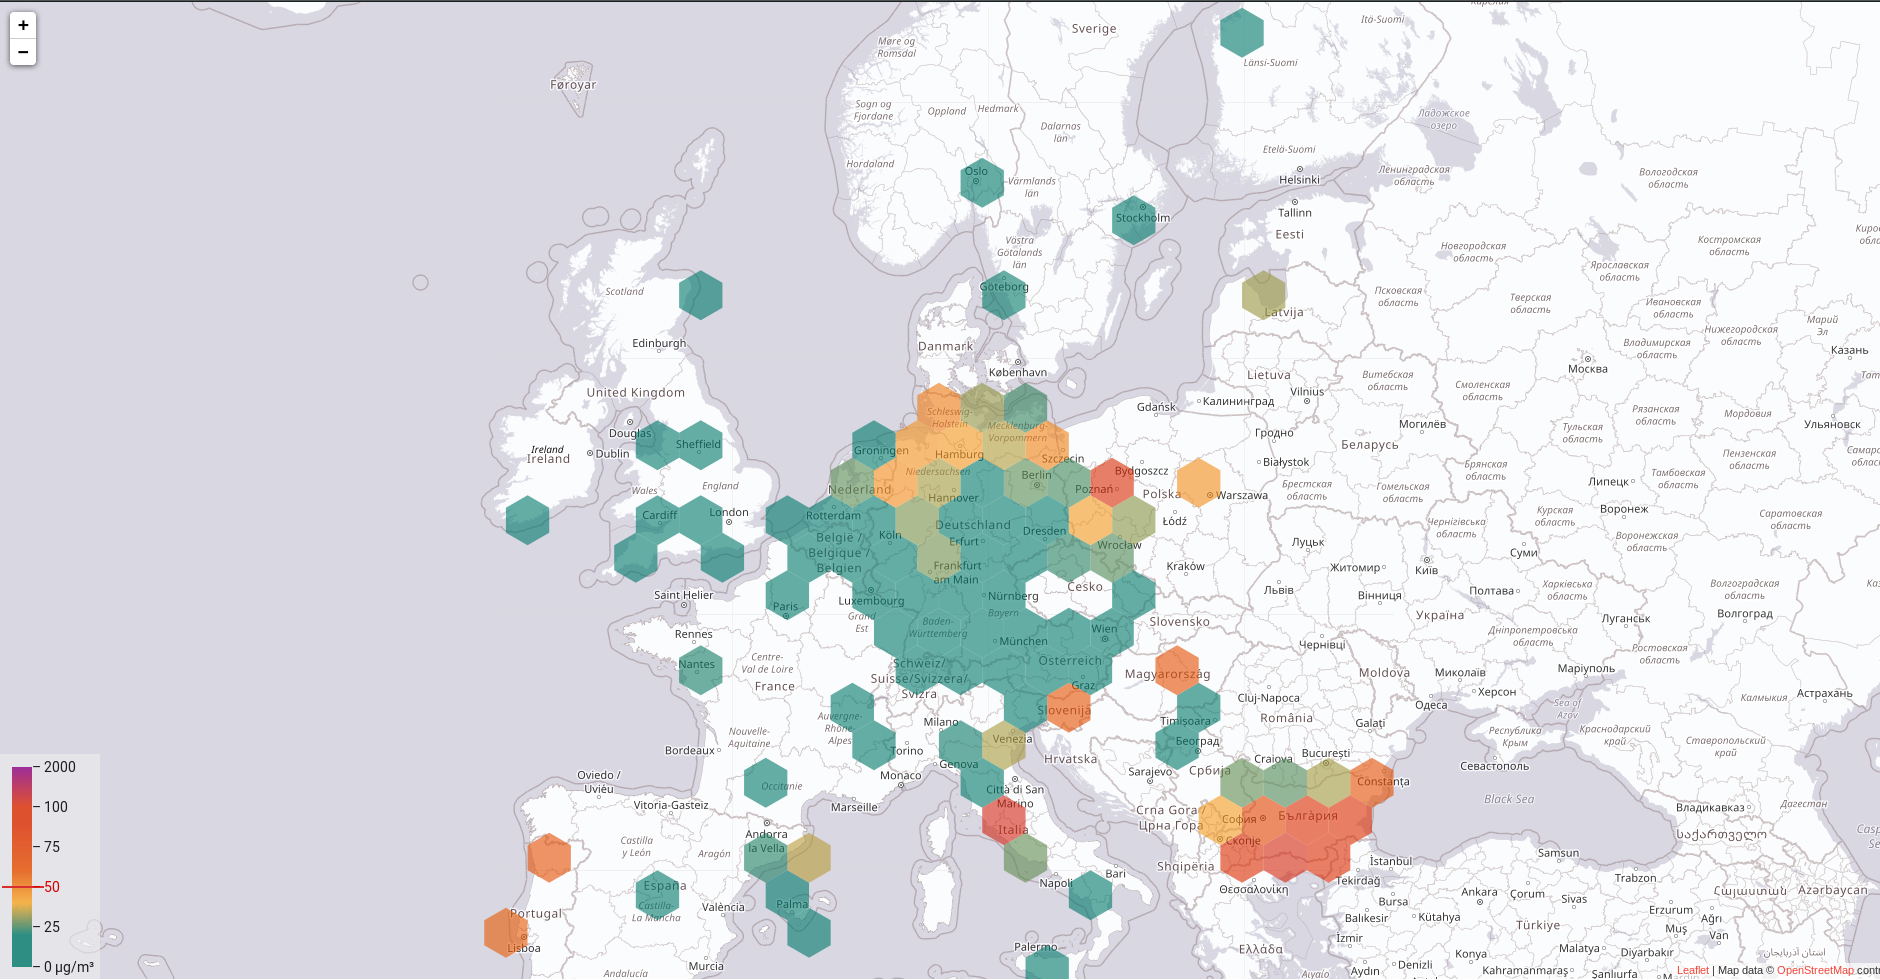
\includegraphics[width=\textwidth]{../screenshots/luftdaten-zoom-e.png}
  \end{center}
\end{frame}
\subsection{Deutschland}
\begin{frame}{\href{http://hannover.maps.luftdaten.info/\#6/52.373/10.005}{luftdaten.info}}
  \begin{center}
    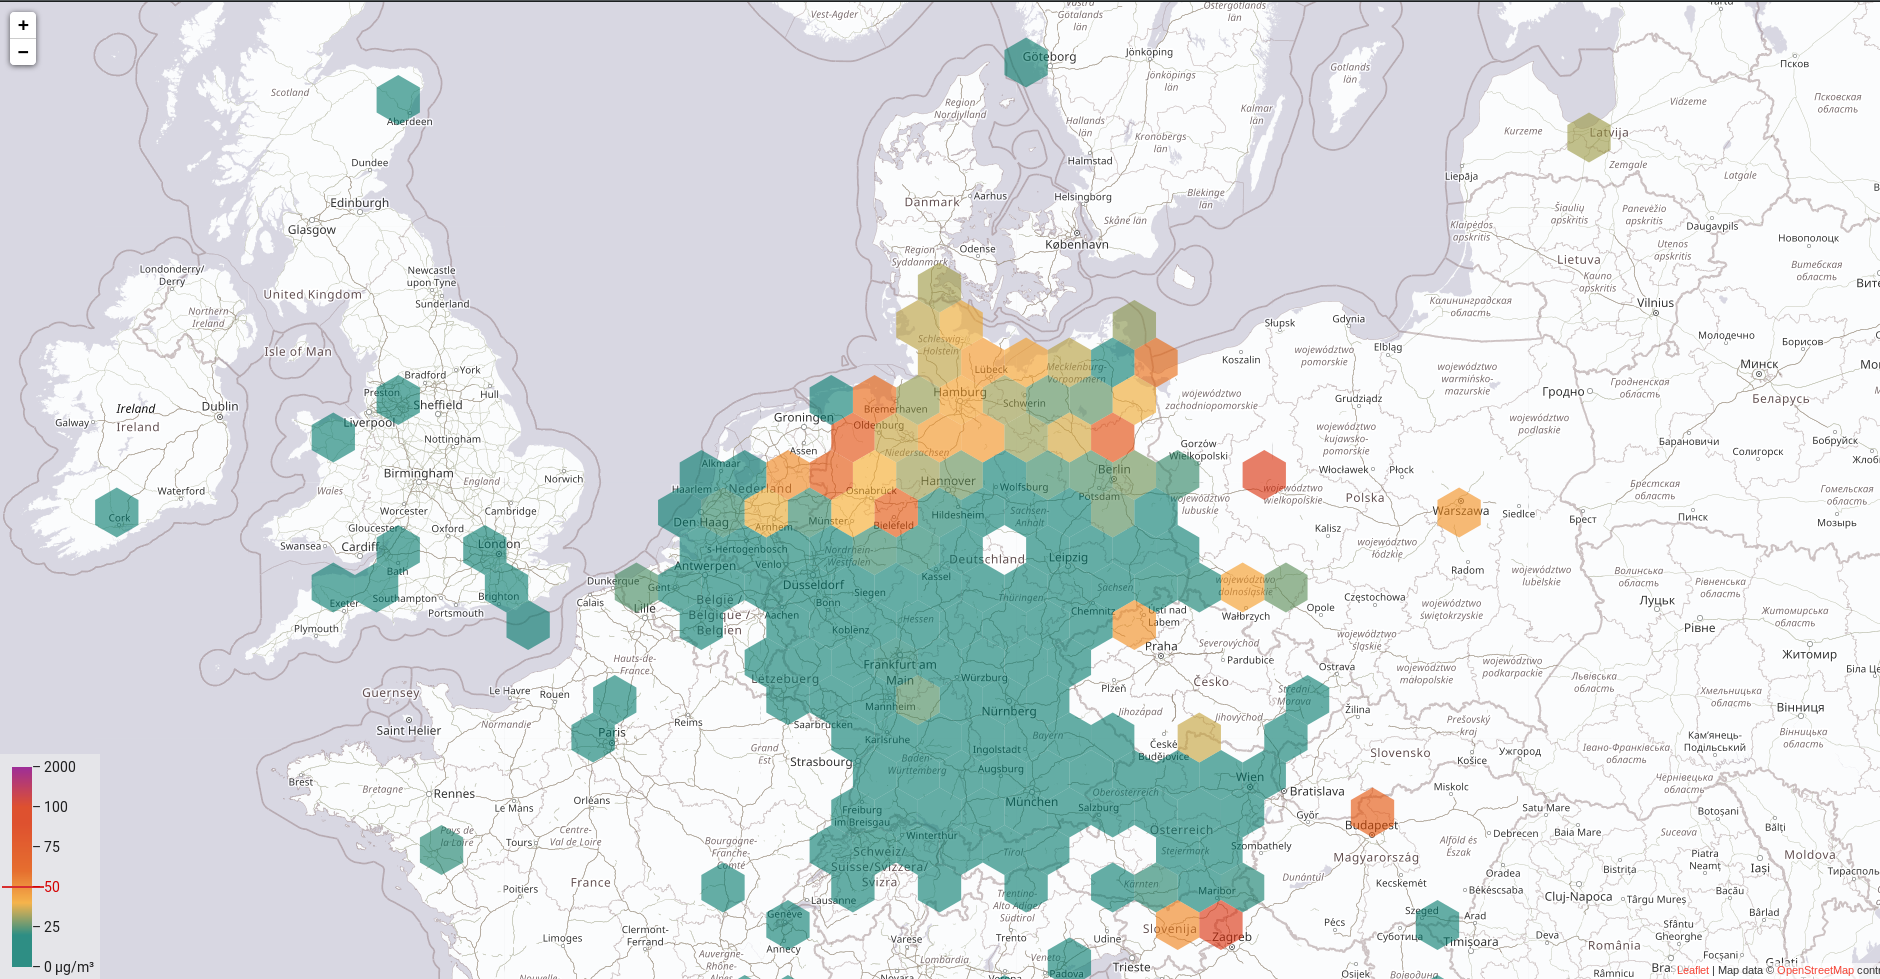
\includegraphics[width=\textwidth]{../screenshots/luftdaten-zoom-f.png}
  \end{center}
\end{frame}
\subsection{Norddeutschland}
\begin{frame}{\href{http://hannover.maps.luftdaten.info/\#8/52.373/10.005}{luftdaten.info}}
  \begin{center}
    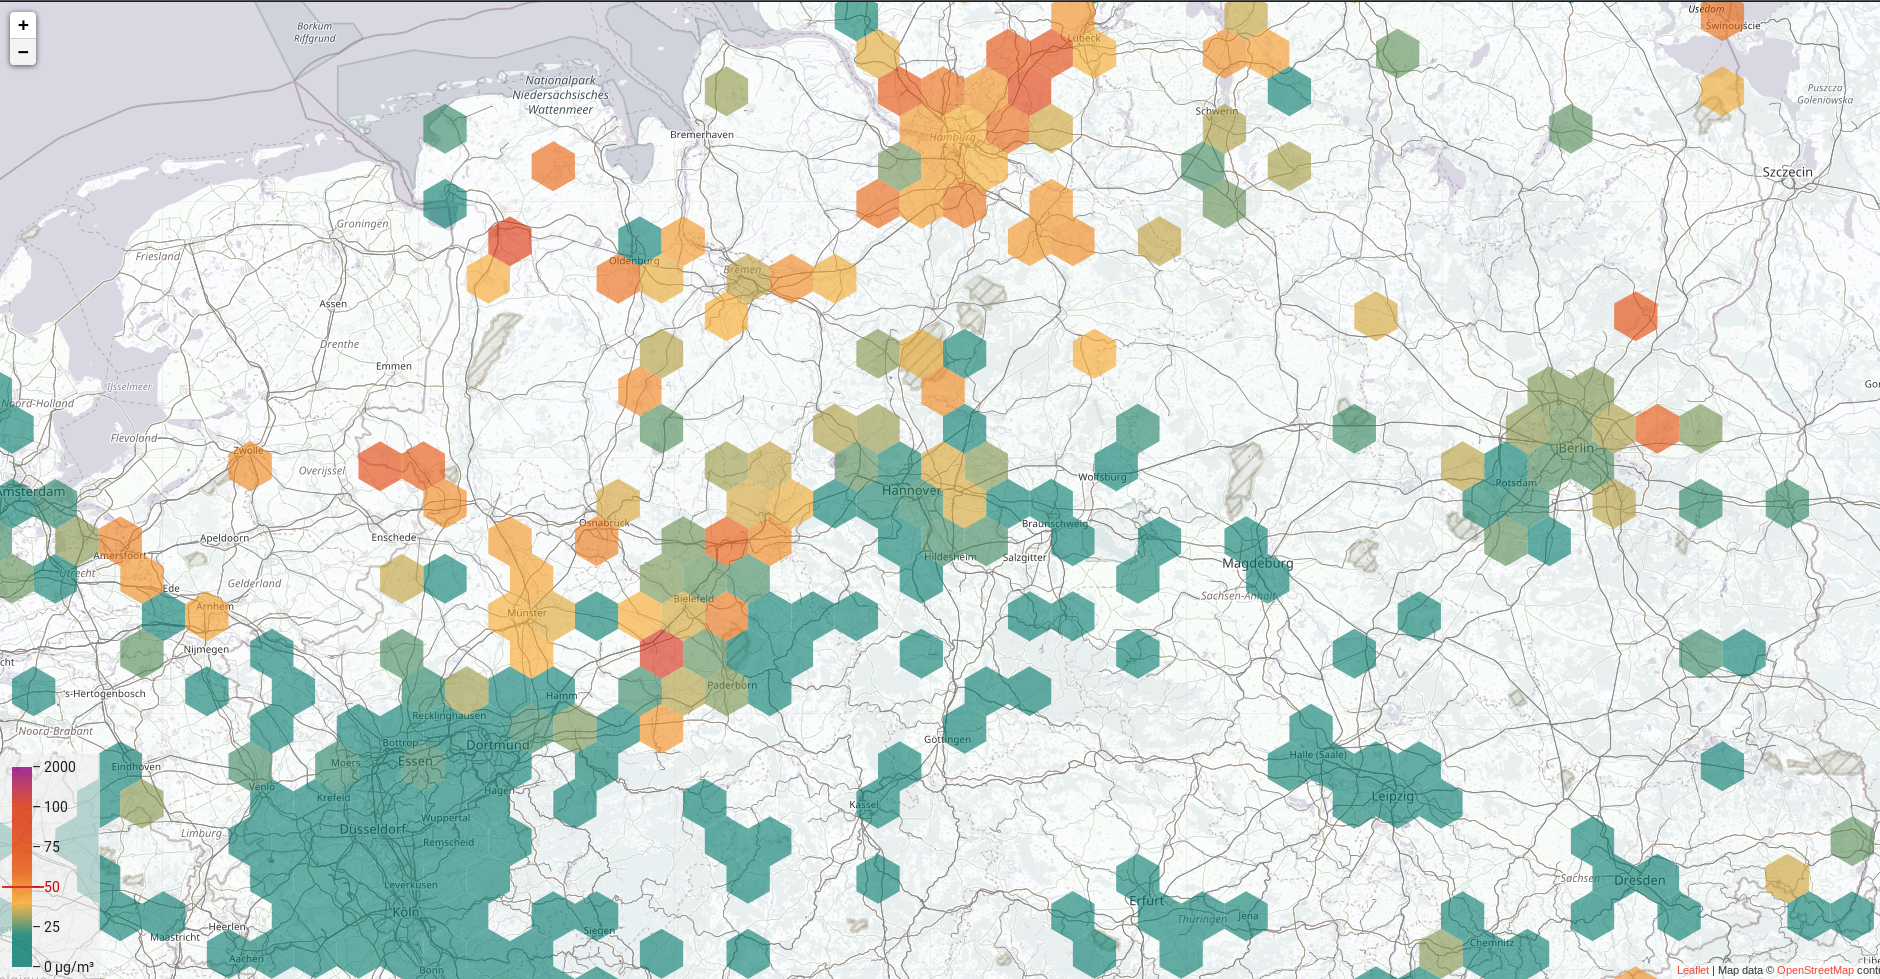
\includegraphics[width=\textwidth]{../screenshots/luftdaten-zoom-d.png}
  \end{center}
\end{frame}
\subsection{Hannover}
\begin{frame}{\href{http://hannover.maps.luftdaten.info/\#10/52.373/10.005}{luftdaten.info}}
  \begin{center}
    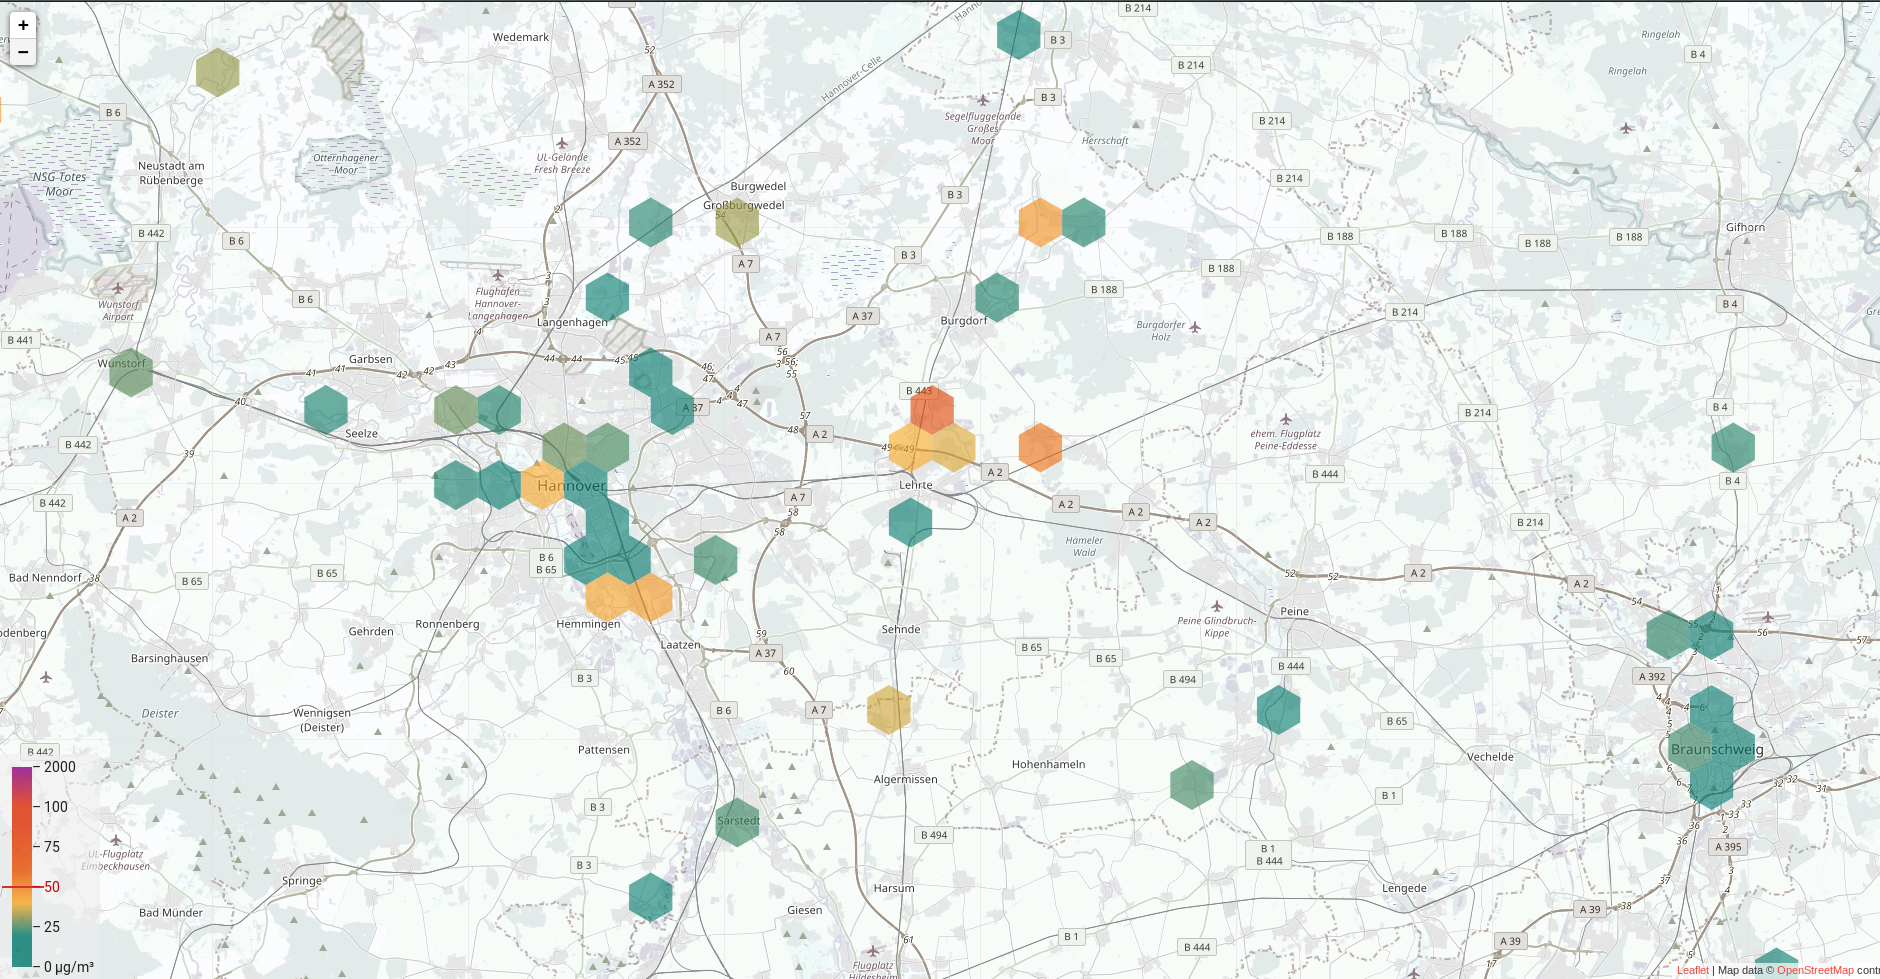
\includegraphics[width=\textwidth]{../screenshots/luftdaten-zoom-b.png}
  \end{center}
\end{frame}
\subsection{Lehrte}
\begin{frame}{\href{http://hannover.maps.luftdaten.info/\#12/52.373/10.005}{luftdaten.info}}
  \begin{center}
    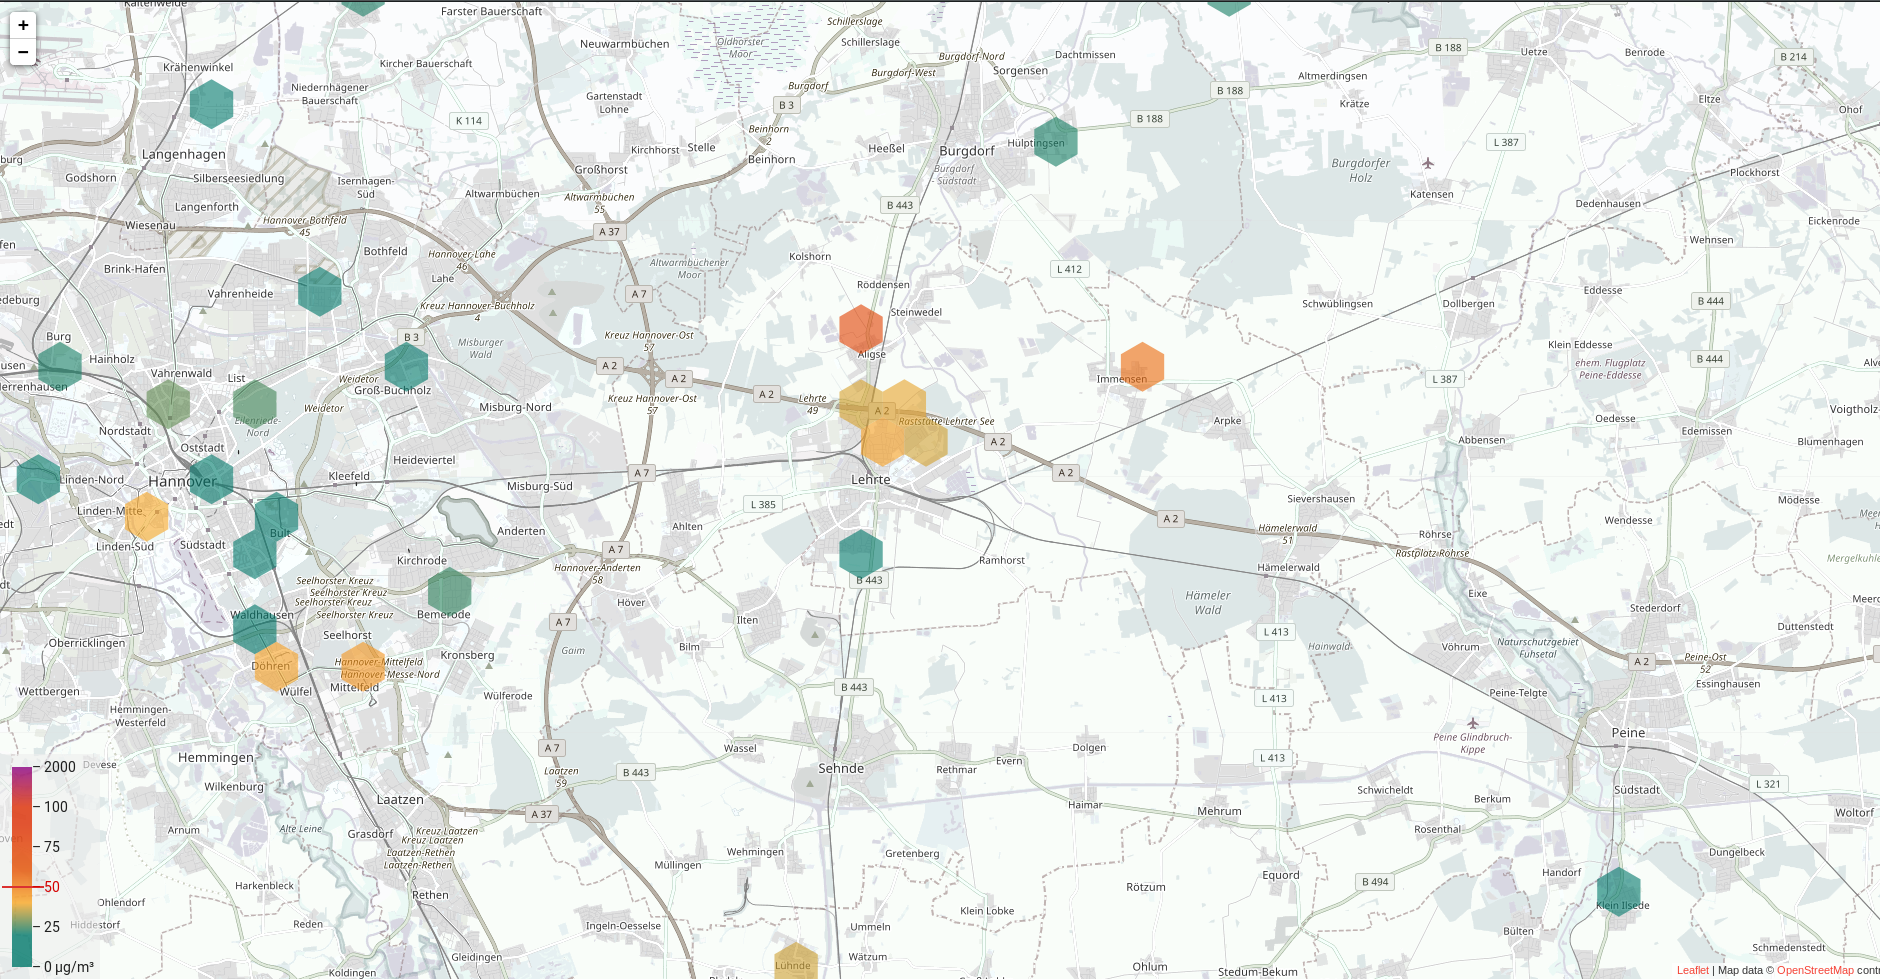
\includegraphics[width=\textwidth]{../screenshots/luftdaten-zoom-a.png}
  \end{center}
\end{frame}

\section{Monate}
\subsection{September}
\begin{frame}{braunschweig}
  \begin{center}
    \includegraphics[width=\textwidth]{../gnuplot/braunschweig-2017-09.png}
  \end{center}
\end{frame}
\begin{frame}{hannover}
  \begin{center}
    \includegraphics[width=\textwidth]{../gnuplot/hannover-2017-09.png}
  \end{center}
\end{frame}
\begin{frame}{lehrte}
  \begin{center}
    \includegraphics[width=\textwidth]{../gnuplot/lehrte-2017-09.png}
  \end{center}
\end{frame}

\subsection{Oktober}
\begin{frame}{braunschweig}
  \begin{center}
    \includegraphics[width=\textwidth]{../gnuplot/braunschweig-2017-10.png}
  \end{center}
\end{frame}
\begin{frame}{hannover}
  \begin{center}
    \includegraphics[width=\textwidth]{../gnuplot/hannover-2017-10.png}
  \end{center}
\end{frame}
\begin{frame}{lehrte}
  \begin{center}
    \includegraphics[width=\textwidth]{../gnuplot/lehrte-2017-10.png}
  \end{center}
\end{frame}

\subsection{November}
\begin{frame}{braunschweig}
  \begin{center}
    \includegraphics[width=\textwidth]{../gnuplot/braunschweig-2017-11.png}
  \end{center}
\end{frame}
\begin{frame}{hannover}
  \begin{center}
    \includegraphics[width=\textwidth]{../gnuplot/hannover-2017-11.png}
  \end{center}
\end{frame}
\begin{frame}{lehrte}
  \begin{center}
    \includegraphics[width=\textwidth]{../gnuplot/lehrte-2017-11.png}
  \end{center}
\end{frame}

\subsection{Dezember}
\begin{frame}{braunschweig}
  \begin{center}
    \includegraphics[width=\textwidth]{../gnuplot/braunschweig-2017-12.png}
  \end{center}
\end{frame}
\begin{frame}{hannover}
  \begin{center}
    \includegraphics[width=\textwidth]{../gnuplot/hannover-2017-12.png}
  \end{center}
\end{frame}
\begin{frame}{lehrte}
  \begin{center}
    \includegraphics[width=\textwidth]{../gnuplot/lehrte-2017-12.png}
  \end{center}
\end{frame}

\subsection{Januar}
\begin{frame}{braunschweig}
  \begin{center}
    \includegraphics[width=\textwidth]{../gnuplot/braunschweig-2018-01.png}
  \end{center}
\end{frame}
\begin{frame}{hannover}
  \begin{center}
    \includegraphics[width=\textwidth]{../gnuplot/hannover-2018-01.png}
  \end{center}
\end{frame}
\begin{frame}{lehrte}
  \begin{center}
    \includegraphics[width=\textwidth]{../gnuplot/lehrte-2018-01.png}
  \end{center}
\end{frame}

\subsection{Quellen}
\begin{frame}{Angaben}
  \begin{enumerate}
  \item OSM
  \item luftdaten
  \item gnuplot
  \item \href{https://www.umwelt.niedersachsen.de/themen/luft/luen/aktuelle_messwerte/archiv/download/}{umwelt.niedersachsen.de Luft Download Archiv}
  \item ...
  \end{enumerate}
\end{frame}

\end{document}

